\documentclass[]{article}
\usepackage{graphicx}
\usepackage{indentfirst}
\usepackage{clrscode3e}
\setlength{\parindent}{0pt}
%opening
\title{CLRS Exercise}
\author{Tongda Xu}

\begin{document}

\maketitle
\section{7}
\subsection{7.3}
\subsubsection{a}
This is certain concerning the $Randomized$ procedure, the probability of any index $i$ is chosen from $[0,n-1]$is:\\
$Pr(pivot = i) = \frac{1}{n}$\\
$E(X_{i}) = 1*Pr(pivot = i) + 0*Pr(pivot \neq i) = \frac{1}{n}$

\subsubsection{b}
It is certain that if $ith$ element is chosen as pivot, $Random-Parition$ cost $\Theta(n)$ time, and it will call $QuickSort[1, q-1], QuickSort[q+1, n]$ recursively.\\
Concerning only the first $Parition$, this would be the result:\\
$E(T(n)) = \Sigma_{i=1}^{n}Pr(pivot = i)(T(i-1) + T(n-i) + \Theta(n))\\
 = \Sigma_{i=1}^{n}X_{i}(T(i-1) + T(n-i) + \Theta(n))$
 
\subsubsection{c}
Concerning $X_{i} = \frac{1}{n}\\
E(T(n)) = \Sigma_{i=1}^{n}\frac{1}{n}(T(i-1) + T(n-i) + \Theta(n))\\
= \Sigma_{i=1}^{n}\frac{1}{n}T(i-1) + \Sigma_{i=1}^{n}\frac{1}{n}T(n-i) + \Sigma_{i=1}^{n}\frac{1}{n}\Theta(n)\\
= \frac{2}{n}\Sigma_{i=1}^{n-1}T(i) + \Theta(n)$

\subsubsection{d}
$\Sigma_{k=2}^{n-1}klgk \\
\le lg\frac{n}{2}\Sigma_{k=2}^{\frac{n}{2}}k + lgn\Sigma_{k=\frac{n}{2}}^{n-1}k\\
= lgn\Sigma_{k=2}^{n-1}k - lg2\Sigma_{k=2}^{\frac{n}{2}}k\\
= lgn\frac{(n+1)(n-2)}{2} - \frac{(\frac{n}{2} + 2)(\frac{n}{2}-1)}{2}\\
\le lgn\frac{n^2}{2} - \frac{n^2}{8}$\\
by Calculus, we have:\\
$(\frac{1}{2}x^2lgx - \frac{1}{4}x^2)|_{1}^{n-1} \le E(T(n)) \le (\frac{1}{2}x^2lgx - \frac{1}{4}x^2)|_{2}^{n}$

\subsubsection{e}
Proof of $E(T(n)) = O(nlgn)$:\\
Assume that $\forall k \in [1, n-1], \exists c, E(T(k)) \le cklgk - \Theta(k)$\\
For $k = n, E(T(n)) \le \frac{n}{2}c(lgn\frac{n^2}{2} - \frac{n^2}{4} - \Theta (n^2)) + \Theta(n) \le cnlgn - \Theta(n) $\\
Proof of $E(T(n)) =\Omega(nlgn)$:\\
Assume that $\forall k \in [1, n-1], \exists c, E(T(k)) \ge cklgk + \Theta(k)$\\
For $k = n, E(T(n)) \ge \frac{n}{2}c(lgn\frac{(n-1)^2}{2} - \frac{(n-1)^2}{4} + \Theta(n^2)) + \Theta(n) \ge cnlgn + \Theta(n)$\\
$\rightarrow E(T(n)) = \Theta(nlgn)$

\subsection{7.5}

\subsubsection{a}
From counting Theorem, it could be noticed that:\\
$p_{i} = \frac{(i-1)(n-i)}{C_{n}^{3}} = \frac{6(i-1)(n-i)}{n(n-1)(n-2)}$

\subsubsection{b}
$Pr(i = medium) (normal) = \frac{1}{n}\\
Pr(i = medium) (3part) = \frac{6(\frac{1}{2}n-1)(n-\frac{1}{2}n)}{n(n-1)(n-2)} = \frac{3}{2}\frac{1}{n}\\
Pr(3part) - Pr(normal) = \frac{1}{2}\frac{1}{n}$

\subsubsection{c}
Consider $f_{diff}= {\int }_{\frac{n}{3}}^{\frac{2}{3}n} (\frac{6(i-1)(n-i)}{n(n-1)(n-2)} - \frac{1}{n})di\\
 = \frac{(-2i^3 + 3(n+1)i^2 - 6ni - (n-1)(n-2)i)|_{i = \frac{1}{3}n}^{i = \frac{2}{3}n}}{n(n-1)(n-2)}\\
{lim}_{n\to \infty} f_{diff} = \frac{4}{27}$

\subsubsection{d}
Consider we are so lucky that each partition we choose the median:\\
In the Iteration tree, we have:\\
$ T(n)=\left\{
\begin{array}{lcl}
c       &      & {n = 1}\\
2T(\frac{1}{2}n) + n     &      & {n > 1}\\
\end{array} \right. $\\
The $\Omega(nlgn)$ is kept even in best case.

\section{8}
\subsection{8.1-1}
n-1 times, since we need n elements to formulate
\subsection{8.1-2}
$\Sigma_{1}^{n}lgk < \int_{1}^{n+1}lgkdk = (klgk - k)_{1}^{n} = (nlgn - n) - (0 - 1) = nlgn -n + 1 $
\subsection{8.1-3}

$ \leftrightarrow $ proof at least half of branch is longer than h
\\Consider a decision tree with $n!/2$ elements

$\leftrightarrow$ proof at least half of branch is longer than h
\\Consider a decision tree with $n!/n$ elements

$\leftrightarrow$ proof at least half of branch is longer than h
\\Consider a decision tree with $n!/2^n$ elements, this is not significant enough and could leave only $\Omega (lg\frac{n!}{2^n}) = \Omega(nlgn - n) = \Omega (nlgn)$ elements

\subsection{8.2-4}
Consider a trim version of counting sort, build the $C$ map up and query directly:
\begin{codebox}
	\Procname{$\proc{Counting-sort-trim($A, k$)}$}
	\li $C []$
	\li \For $i \gets 0$ \To $k$
	\li		\Do $C[i] = 0$
	\End
	\li \For $j \gets 1$ \To $A.length$
	\li		\Do $C[A[j]]++$
	\End
	\li \For $m \gets 1$ \To $k$
	\li		\Do $C[m] += C[m-1]$
	\End
	\li \Return $C[m]$
\end{codebox}

\begin{codebox}
	\Procname{$\proc{Direct-Quert($A, k, a, b$)}$}
	\li $C = \proc{Counting-sort-trim($A, k$)}$
	\li \If $a < 1$
	\li \Then \Return $C[b]$
	\li \Else \Return $C[b] - C[a-1]$
\end{codebox}

\subsection{8.3-4}
First, with $O(n)$ time: convert n numbers $k_{10}$ into $k_{n}$ which has 3 digits.\\
Second, with $O(d(n+n))$ time ($Lemma8.3$): Radix sort n 3-digit numbers with each digits take up to n possible values.

\begin{codebox}
	\Procname{$\proc{digitsConvert($X$)}$}
	\li $result []$
	\li \For $i \gets 2$ \Downto $0$
	\li		\Do $result[i] = X/n^i$
	\li			$X = X \bmod{n^i}$
	\End
	\li \Return $result$
\end{codebox}

\begin{codebox}
	\Procname{$\proc{sort($A,x$)}$}
	\li $result []$
	\li \For each $S$ in $A$
	\li		\Do $S =\proc{digitsConvert($S$)}$
	\End
	\li \proc{radix-sort($A,x$)}
\end{codebox}

\section{9}

\subsection{9.1}
\subsubsection{a}

Sorting: $\proc{Merge-sort($A$)}$ in worst case $O(nlgn)$\\
Query: $\proc{call-by-rank($A,k$)}$ i times in worst case $O(i)$, here we assume manipulating $O(n)$ space cost $O(n)$ time.

\subsubsection{b}

Building: $\proc{build-map-heap($A$)}$ in worst case $O(n)$\\
Query: calling $\proc{Extra-max($A,k$)}$ i times in worst case $O(ilgn)$

\subsubsection{c}

Selecting: $\proc{select($A, i$)}$ in worst case $O(n)$\\
Sorting:  $\proc{Merge-sort($A^{'}$)}$ in worst case $O(ilgi)$

\section{11}

\subsection{11.2}
\subsubsection{a}

Consider for a ball i fall into a specific bucket $Pr(i) = \frac{1}{n}$\\
Then consider Binomial Distribution, $Pr(k) = C_{n}^{k}Pr(i)^{k}(1-Pr(i))^{n-k}$

\subsubsection{b}

Consider random picking a slot, the probability of that slot is maximum is $Pr_{max} = \frac{1}{n}$, and it contains k elements $Q_{k}$. for conditional probability, we have:\\
$P_{k} = Pr_{i=k|max} = \frac{Pr(i=k \cap max)}{Pr_{max}} \le \frac{Pr(i=k)}{Pr_{max}} = nQ_{k}$

\subsubsection{c}

Proof:\\
$Q_k = (\frac{1}{n})^k(\frac{n-1}{n})^{n-k}C_{n}^{k} \\
= \frac{(n-1)^{n-k}}{n^n} \frac{\Pi_{0}^{k-1}n-k}{k!} \\
\le \frac{n^n}{n^n} \frac{1}{k!}\\
= \frac{e^k}{k^k} \frac{1}{k^{\frac{1}{2}} (1+\Theta(\frac{1}{n}))}\\
\le \frac{e^k}{k^k}$

\subsubsection{d}

Proof for $Q_{k_{0}}$: \\
$Q_{k_{0}} = \frac{e^{(\frac{clgn}{lglgn})}}{(\frac{clgn}{lglgn}) ^ {\frac{clgn}{lglgn}}}\\
= \frac{n^{\frac{clg\frac{e}{c}}{lglgn}}}{\frac{n^c}{n^{\frac{clglglgn}{lglgn}}}} = n^{\frac{clg\frac{e}{c} + clglglgn}{lglgn} - c}$\\
It would not take effort to notice that since ${lim}_{n\to \infty}\frac{clg\frac{e}{c} + clglglgn}{lglgn} =0\\
\forall c > 3+\epsilon, Q_{k_{0}} = O(\frac{1}{n^3}) $\\
And $P_{k} \le nQ_{k} \rightarrow P_{k} = O(\frac{1}{n^2})$

\subsubsection{e}

$E(M) = \Sigma_{M = 1}^{n} M Pr(M) < nPr(M>\frac{clgn}{lglgn}) + \frac{clgn}{lglgn}Pr(M \le \frac{clgn}{lglgn})\\$
A stronger conclusion to note: \\
$E(M) = \Sigma_{M = 1}^{n} M Pr(M) < MPr(M>\frac{clgn}{lglgn}) + \frac{clgn}{lglgn}Pr(M \le \frac{clgn}{lglgn})\\
\le \int_{\frac{clgn}{lglgn}}^{\infty}\frac{1}{n}dn + 1*\frac{clgn}{lglgn} \\
= lg (\frac{clgn}{lglgn}) + \frac{clgn}{lglgn}\\ = O(\frac{clgn}{lglgn})$

\section{15}

\subsection{15.1-1}
$2^n -1 = \Sigma_{j = 0}^{n-1} 2^j $
\subsection{15.1-2}
Do not know how!

\subsection{15.1-3}
See Code

\subsection{15.1-4}
See Code

\subsection{15.1-5}
See Code

\subsection{15.2-1}
See Code

\subsection{15.2-2}
See Code

\subsection{15.2-3}

Assume that $\forall k \le n-1, T(k) \ge c2^k$\\
Then $T(n) = \Sigma_{k = 1}^{n-1} T(k)T(n-k) = (n-1)c^22^n > c2^n$\\
So $T(n) = \Omega (n), \omega(n)$

\subsection{15.2-4}
See Figure ~\ref{fig:15.2-4}

\begin{figure}
	\centering
	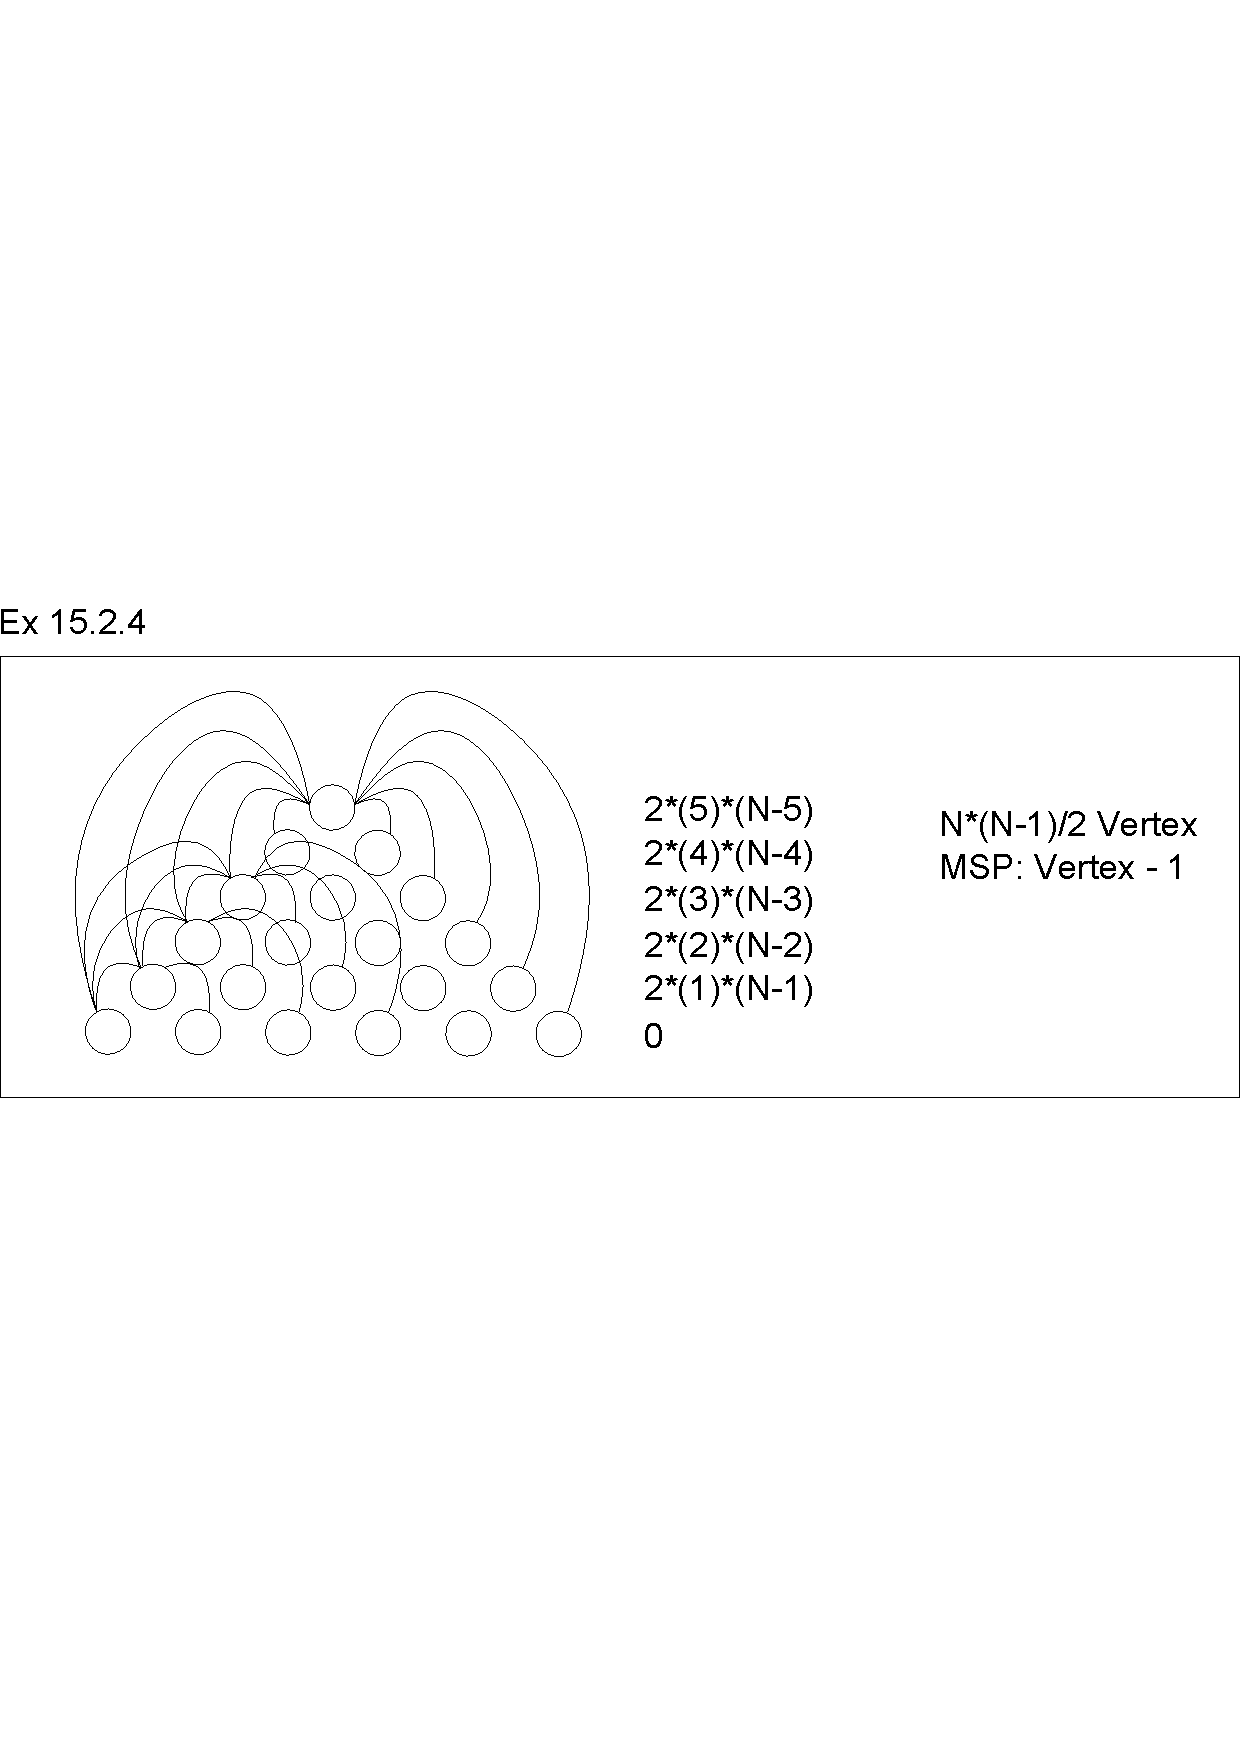
\includegraphics[width=0.8\linewidth]{1524}
	\caption{15.2-4}
	\label{fig:15.2-4}
\end{figure}

\subsection{15.2-5}
For each level $h(i) = i (n-i)$\\
For tree $T(n) = 2\Sigma_{i = 1}^{n-1}i(n-i)
\\ = \frac{3n^3 + 3n^2}{3} - \frac{2n^3 + 3n^2 +n}{3}
\\ = \frac{n^3 - n }{3}$

\subsection{15.2-6}
Assume that $\forall k \le n-1, N(k) = k-1$\\
Then $N(n) = N(n-1) + 1$\\
So $N(n) = n-1$

\subsection{15.3-1}
running through: $T(n) = n*P_{n}^{n} = n*n! > 4^{n}$\\
running recursion: $T(n) = 2\Sigma_{i=1}^{n-1}4^i + n = \frac{8}{3}4^{n-1} + n \le 4^n$\\
running through takes longer

\subsection{15.3-2}
no overlapping subproblem call

\subsection{15.3-3}
Yes

\subsection{15.3-4}
Do not know how!

\subsection{15.4-1}
See code

\subsection{15.4-2}
See code

\subsection{15.4-3}
See code

\subsection{15.1}

\begin{codebox}
	\Procname{$\proc{LSP($s, t, G$)}$}
	\li $r = G,size()$
	\li $DPs[r] = 0$
	\li $DPr[r] = path(s,t)$
	\li $max = -\infty$
	\li \For $i \gets 1$ \To $r$
	\li		\Do $max (DPs[j] + DPr[r-j] + what)$
	\End
	\li \Return $max$
\end{codebox}

\subsection{15.1}
%subpriblem? vector<string> ()

\end{document}
